\begin{figure*}[t!]%
\definecolor{hair}{gray}{1}%
\definecolor{head}{rgb}{.85,.85,1}%
\definecolor{body}{rgb}{.5,.8,.5}%
\definecolor{tail}{rgb}{.55,.55,.55}%
\centering
\begin{subfigure}[t]{.475\linewidth}
\centering
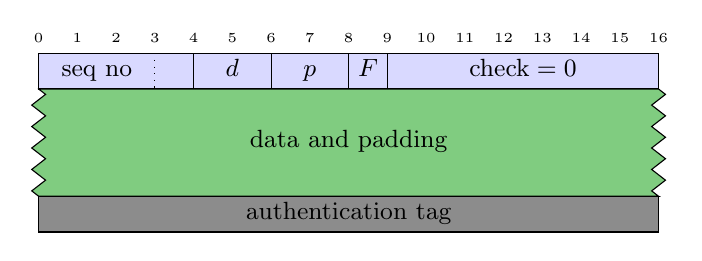
\begin{tikzpicture}[x=1.75pt,y=3ex]
\small
{\tiny
\foreach \x/\l in {0/0, 8/1, 16/2, 24/3, 32/4, 40/5, 48/6, 56/7,
                   64/8, 72/9, 80/10, 88/11, 96/12, 104/13, 112/14,
                   120/15, 128/16}
  \node [above] at (\x,0.1) {\l} ;
}
\filldraw [fill=head] (0,0) rectangle (128,-1) ;
\draw (32,0) -- (32,-1)
      (48,0) -- (48,-1)
      (64,0) -- (64,-1)
      (72,0) -- (72,-1) ;
\draw [dotted] (24, 0) -- (24, -1) ;
\node [anchor=mid,inner sep=0pt, outer sep=0pt] at (12,  -0.5) {seq no} ;
\node [anchor=mid,inner sep=0pt, outer sep=0pt] at (40,  -0.5) {$d$} ;
\node [anchor=mid,inner sep=0pt, outer sep=0pt] at (56,  -0.5) {$p$} ;
\node [anchor=mid,inner sep=0pt, outer sep=0pt] at (68,  -0.5) {$F$} ;
\node [anchor=mid,inner sep=0pt, outer sep=0pt] at (100, -0.5)
   {$\mbox{check} = 0$} ;
\filldraw [fill=body,decoration={zigzag,segment length=2ex}]
  (128,-1) decorate { -- (128,-4) } -- (0,-4) decorate { -- (0,-1) } -- cycle;
\node [anchor=mid,inner sep=0pt, outer sep=0pt] at (64,-2.5)
  {data and padding} ;
\filldraw [fill=tail] (0,-4) rectangle (128,-5) ;
\node [anchor=mid,inner sep=0pt, outer sep=0pt] at (64,-4.5)
  {authentication tag} ;
\end{tikzpicture}%
\caption{Blocks consist of a header, up to $2^{15}-1$ bytes each of
  data and padding, and an authentication tag. $d$:~data length;
  $p$:~padding length; $F$:~function code.  $d+p$ is not required to
  be a multiple of 16.\label{f:block}}
\end{subfigure}
\quad
\begin{subfigure}[t]{.47\linewidth}
\centering
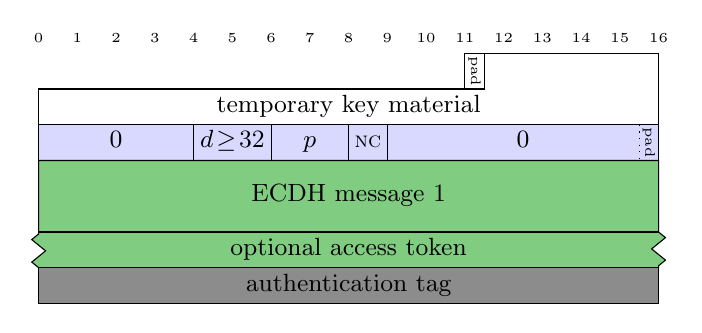
\begin{tikzpicture}[x=1.75pt,y=3ex]
\small
{\tiny
\foreach \x/\l in {0/0, 8/1, 16/2, 24/3, 32/4, 40/5, 48/6, 56/7,
                   64/8, 72/9, 80/10, 88/11, 96/12, 104/13, 112/14,
                   120/15, 128/16}
  \node [above] at (\x,2.1) {\l} ;
}
\filldraw [fill=hair] (0,1) -- (0,0) -- (128,0) -- (128,2)
                            -- (88,2) -- (88,1) -- cycle;
\draw (88,1) -- (92,1) -- (92,2) ;
\node [rotate=-90] at (90,  1.5) {\tiny pad};
\node [anchor=mid,inner sep=0pt, outer sep=0pt] at (64,0.5)
 {temporary key material};
\filldraw [fill=head] (0,0) rectangle (128,-1) ;
\draw (32,0) -- (32,-1)
      (48,0) -- (48,-1)
      (64,0) -- (64,-1)
      (72,0) -- (72,-1) ;
\draw [dotted] (124,0) -- (124,-1) ;
\node [anchor=mid,inner sep=0pt, outer sep=0pt] at (16,  -0.5) {0} ;
\node [anchor=mid,inner sep=0pt, outer sep=0pt] at (40,  -0.5) {$d\!\ge\!32$} ;
\node [anchor=mid,inner sep=0pt, outer sep=0pt] at (56,  -0.5) {$p$} ;
\node [anchor=mid,inner sep=0pt, outer sep=0pt] at (68,  -0.5)
  {\footnotesize\scshape nc} ;
\node [anchor=mid,inner sep=0pt, outer sep=0pt] at (100, -0.5) {0} ;
\node [rotate=-90] at (126, -0.5) {\tiny pad};
\filldraw [fill=body,decoration={zigzag,segment length=2.1ex}]
    (0,-1) -- (128,-1) -- (128,-3) decorate { -- (128,-4) }
    -- (0,-4) decorate { -- (0,-3) } -- cycle;
\node [anchor=mid,inner sep=0pt, outer sep=0pt]
  at (64,-2) {ECDH message 1};
\node [anchor=mid,inner sep=0pt, outer sep=0pt]
  at (64,-3.5) {optional access token};
\draw (0,-3) -- (128,-3) ;
\filldraw [fill=tail] (0,-4) rectangle (128,-5) ;
\node at (64,-4.5) {authentication tag} ;
\end{tikzpicture}
\caption{A new-link request consists of a Möller key encapsulation,
  followed by a block encrypted with the temporary key material.  Four
  padding bits are copied into the “check” field to make them
  non-malleable.\label{f:cnewlink}}
\end{subfigure}
\quad
\begin{subfigure}[t]{.47\linewidth}
\centering
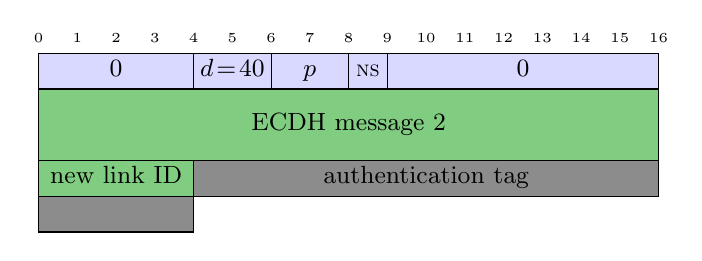
\begin{tikzpicture}[x=1.75pt,y=3ex]
\small
{\tiny
\foreach \x/\l in {0/0, 8/1, 16/2, 24/3, 32/4, 40/5, 48/6, 56/7,
                   64/8, 72/9, 80/10, 88/11, 96/12, 104/13, 112/14,
                   120/15, 128/16}
  \node [above] at (\x,0.1) {\l} ;
}
\filldraw [fill=head] (0,0) rectangle (128,-1) ;
\draw (32,0) -- (32,-1)
      (48,0) -- (48,-1)
      (64,0) -- (64,-1)
      (72,0) -- (72,-1) ;
\node [anchor=mid,inner sep=0pt, outer sep=0pt] at (16,  -0.5) {0} ;
\node [anchor=mid,inner sep=0pt, outer sep=0pt] at (40,  -0.5) {$d\!=\!40$} ;
\node [anchor=mid,inner sep=0pt, outer sep=0pt] at (56,  -0.5) {$p$} ;
\node [anchor=mid,inner sep=0pt, outer sep=0pt] at (68,  -0.5)
  {\footnotesize\scshape ns} ;
\node [anchor=mid,inner sep=0pt, outer sep=0pt] at (100, -0.5) {0} ;
\fill [fill=body] (0,-1) -- (128,-1) -- (128,-3) -- (32,-3) -- (32,-4)
               -- (0,-4) -- cycle;
\fill [fill=tail] (32,-3) rectangle (128,-4) (0,-4) rectangle (32,-5) ;
\draw (0,-1) rectangle (128,-3)
      (0,-3) rectangle (128,-4)
      (0,-4) -- (0,-5) -- (32,-5) -- (32,-3) ;
\node [anchor=mid,inner sep=0pt, outer sep=0pt] at (64,-2)
  {ECDH message 2};
\node [anchor=mid,inner sep=0pt, outer sep=0pt] at (16,-3.5) {new link ID};
\node [anchor=mid,inner sep=0pt, outer sep=0pt] at (80,-3.5)
  {authentication tag} ;
\end{tikzpicture}
\caption{A new-link response is a normal block, encrypted with the
  temporary key material.\label{f:snewlink}}
\end{subfigure}
\quad
\begin{subfigure}[t]{.475\linewidth}
\centering
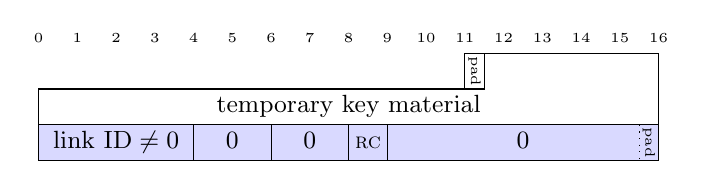
\begin{tikzpicture}[x=1.75pt,y=3ex]
\small
{\tiny
\foreach \x/\l in {0/0, 8/1, 16/2, 24/3, 32/4, 40/5, 48/6, 56/7,
                   64/8, 72/9, 80/10, 88/11, 96/12, 104/13, 112/14,
                   120/15, 128/16}
  \node [above] at (\x,2.1) {\l} ;
}
\filldraw [fill=hair] (0,1) -- (0,0) -- (128,0) -- (128,2)
                            -- (88,2) -- (88,1) -- cycle;
\draw (88,1) -- (92,1) -- (92,2) ;
\node [rotate=-90] at (90,  1.5) {\tiny pad};
\node [anchor=mid,inner sep=0pt, outer sep=0pt] at (64,0.5)
 {temporary key material};
\filldraw [fill=head] (0,0) rectangle (128,-1) ;
\draw (32,0) -- (32,-1)
      (48,0) -- (48,-1)
      (64,0) -- (64,-1)
      (72,0) -- (72,-1) ;
\draw [dotted] (124,0) -- (124,-1) ;
\node [anchor=mid,inner sep=0pt, outer sep=0pt] at (16,  -0.5)
  {$\mbox{link ID} \ne 0$} ;
\node [anchor=mid,inner sep=0pt, outer sep=0pt] at (40,  -0.5) {0} ;
\node [anchor=mid,inner sep=0pt, outer sep=0pt] at (56,  -0.5) {0} ;
\node [anchor=mid,inner sep=0pt, outer sep=0pt] at (68,  -0.5)
  {{\footnotesize\scshape rc}} ;
\node [anchor=mid,inner sep=0pt, outer sep=0pt] at (100, -0.5) {0} ;
\node [rotate=-90] at (126, -0.5) {\tiny pad};
\end{tikzpicture}%
\caption{A reconnection request is just a key encapsulation and a
  modified header. The link ID replaces the sequence number, $d$ and
  $p$ must be zero, and there is no authentication tag.\label{f:creconn}}
\end{subfigure}
\caption{Message formats before steganography.  Background shading
  indicates encryption mode.  {\color{head}$\blacksquare$}:~header
  encryption; {\color{body}$\blacksquare$}:~GCM encryption;
  {\color{tail}$\blacksquare$}:~GCM authentication tag;
  {$\square$}:~Möller key encapsulation.  There are 16 bytes per row
  of each diagram.\label{f:msgfmt}}
\end{figure*}
